\chapter{Analysis of waveguide general approach}
In previous chapters, we investigated a structure called a parallel plane waveguide. If we are having two conducting boundaries, we saw that the electromagnetic energy can propagate between these two boundaries in the form of some definite electric and magnetic field patterns which are called modes. We also try to visualize the propagation of electromagnetic waves between these two boundaries as a superposition of uniform plane waves.

This understanding of modal propagation in terms of the uniform plane wave gives you a correct picture of how the modes are established inside a waveguide. However, this approach that visualises a modal pattern in terms of the fields of a uniform plane wave is always not as easy as we saw in terms of the parallel plane waveguide. In a parallel plane waveguide, since the medium still was infinite at least parallel to the conducting boundaries, we still could use or visualize the uniform plane wave propagating between the boundaries.

However, if we have a structure, like a pipe kind of structure; whether a rectangular pipe or circular pipe or a pipe of arbitrary shape and if I want to find out how the electromagnetic energy is going to propagate inside this structure, it will be extremely difficult to visualize the propagation in terms of a superposition of uniform plane wave and those situations. We develop a mathematical framework and try to solve the problem of electromagnetic wave propagation in structure using that general mathematical formulation.

In this chapter, we develop a general framework for analyzing wave propagation inside an arbitrary waveguide. And then, whatever result we get mathematically, we will try to correlate these results with what we have got for parallel plane waveguide which we visualize as a superposition of uniform plane waves. This will give us confidence that the visualization we had in terms of uniform plane waves for the input current gives us much better physical insight into the problem. However, since resolving in the uniform plane wave will not be possible, We develop a general mathematical framework and solve the problems in the following by using an exit general mathematical approach. we analyze a waveguide with the general approach. 

let us say we have an arbitrarily shaped waveguide as shown in figure~\ref{fig:lect37}.
\begin{figure}[h]
\centering
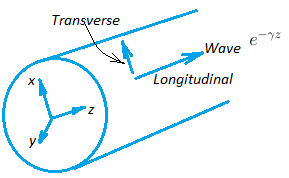
\includegraphics[width=0.7\linewidth]{\pathtoparttwo/graphics/lect37}
\caption{An Arbitrarily Shaped Waveguide}
\label{fig:lect37}
\end{figure}
We can say this is a conducting pipe where the electromagnetic energy can flow along the axis of this pipe, there is wave propagation in the z-direction as shown. At the moment we are not even defining any shape for the cross-section, it could be rectangular, it could be circular or in general, it could be as arbitrarily shaped. The only information needed here is the direction of the wave, which is the z-direction. We develop a general framework starting from the Maxwell equations to show the kind of fields that exists inside the shape and then we will go on to deal with very specific cases of rectangular waveguides and propagation of modal propagation inside the rectangular waveguide. Any electric or magnetic field will be resolved into two components; one is along the wave propagation, called the longitudinal component and the other will be perpendicular to the direction of wave propagation called transverse.
\begin{equation*}
\bar{E} = \bar{E}_\bot + E_z\hat{z}
\end{equation*}
\begin{equation*}
\bar{H} = \bar{H}_\bot + H_z\hat{z}
\end{equation*}
\begin{equation*}
\bar{E}_\bot = E_x\hat{x} + E_y\hat{y}
\end{equation*}
\begin{equation*}
\bar{H}_\bot = H_x\hat{x} + + H_y\hat{y}
\end{equation*}
we define
\begin{equation}
\nabla = \nabla_\bot + \frac{\partial}{\partial z}\hat{z}
\label{eqn:transversegrad}
\end{equation}
where
\begin{equation*}
\nabla_\bot = \frac{\partial}{\partial x}\hat{x} + \frac{\partial}{\partial y}\hat{y}
\end{equation*}
Substituting equation~\ref{eqn:transversegrad} into Maxwell's equations\index{maxwell's equations} for the electric field;
\begin{align*}
\nabla\times\bar{E} = j\omega\mu\bar{H}
\end{align*}
\begin{dmath*}
\left[\nabla_\bot + \frac{\partial}{\partial z}\hat{z}\right]\times(\bar{E}_\bot + E_z\hat{z}) = -j\omega\mu(\bar{H}_\bot + H_z\hat{z})
\end{dmath*}
\begin{dmath*}
\nabla_\bot\times\bar{E}_\bot + \nabla_\bot\times(E_z\hat{z}) + \frac{\partial}{\partial z}\hat{z}\times\bar{E}_\bot + \frac{\partial}{\partial z}\hat{z}\times(E_z\hat{z}) = -j\omega\mu(\bar{H}_\bot + H_z\hat{z})
\end{dmath*}
Taking the transverse and longitudinal components and equating them on two sides
\begin{dmath*}
-j\omega\mu\bar{H}_\bot = \nabla_\bot\times(E_z\hat{z}) + \frac{\partial}{\partial z}\hat{z}\times\bar{E}_\bot
\end{dmath*}
\begin{dmath}
\bar{H}_\bot = -\frac{1}{j\omega\mu} \left[\nabla_\bot\times(E_z\hat{z}) + \frac{\partial}{\partial z}\hat{z}\times\bar{E}_\bot\right]
\label{eqn:transversemag}
\end{dmath}
Similarly, substituting equation~\ref{eqn:transversegrad}  into Maxwell's equation for the magnetic field;
\begin{align*}
\nabla\times\bar{H} = j\omega\epsilon\bar{E}
\end{align*}
\begin{dmath*}
\left[ \nabla_\bot + \frac{\partial}{\partial z}\hat{z} \right] \times (H_\bot + H_z \hat{z}) = \jmath \omega\epsilon (E_\bot + E_z \hat{z})
\end{dmath*}
\begin{dmath*}
\nabla_\bot\times H_\bot + \nabla_\bot\times H_z \hat{z} +  \frac{\partial}{\partial z}\hat{z}\times H_\bot + \frac{\partial}{\partial z}\hat{z}\times H_z \hat{z} = \jmath \omega\epsilon (E_\bot + E_z \hat{z})
\end{dmath*}
Taking the transverse and longitudinal components and equating them on two sides
\begin{dmath}
\bar{E}_\bot = \frac{1}{j\omega\epsilon} \left[\nabla_\bot\times H_z\hat{z} + \frac{\partial}{\partial z}\hat{z}\times\bar{H}_\bot\right]
\label{eqn:transverseele}
\end{dmath}
Substituting equation~\ref{eqn:transversemag} into \ref{eqn:transverseele}
\begin{dmath*}
\bar{E}_\bot = \frac{1}{j\omega\epsilon} \left[\nabla_\bot\times H_z\hat{z} + \frac{\partial}{\partial z}\hat{z}\times \left( -\frac{1}{j\omega\mu} \left[\nabla_\bot\times(E_z\hat{z}) + \frac{\partial}{\partial z}\hat{z}\times\bar{E}_\bot\right] \right)\right] 
\end{dmath*}
Collecting like terms
\begin{dmath}
\omega^2\mu\epsilon\bar{E}_\bot-\frac{\partial}{\partial z}\hat{z}\times\frac{\partial}{\partial z}\hat{z}\times\bar{E}_\bot = \frac{1}{j\omega\epsilon} \left[\nabla_\bot\times H_z\hat{z} - \frac{1}{j\omega\mu}\frac{\partial}{\partial z}\hat{z}\times\nabla_\bot\times E_z \hat{z} \right]
\label{eqn:electricfieldinwg}
\end{dmath}
Identity for vector triple product\index{vector triple product}
\begin{align*}
A\times B\times C = (\bar{A}\cdot\bar{C})\bar{B} - (\bar{A}\cdot\bar{B})\bar{C}
\end{align*}
\begin{dmath*}
\frac{\partial}{\partial z}\hat{z}\times\frac{\partial}{\partial z}\hat{z}\times\bar{E}_\bot = \frac{\partial}{\partial z}\hat{z}\left(\frac{\partial}{\partial z}\hat{z}\cdot\bar{E}_\bot\right)\hat{z} - \left(\frac{\partial}{\partial z}\hat{z}\cdot\frac{\partial}{\partial z}\hat{z}\right)\bar{E}_\bot = -\frac{\partial^2}{\partial z^2}\bar{E}_\bot
\end{dmath*}
where $\dfrac{\partial}{\partial z}\hat{z}\left(\dfrac{\partial}{\partial z}\hat{z}\cdot\bar{E}_\bot\right)\hat{z} = 0$
\begin{dmath*}
\frac{\partial}{\partial z}\hat{z}\times\nabla_\bot\times E_z\hat{z} = \nabla_\bot\left(\frac{\partial}{\partial z}\hat{z}.E_z\hat{z}\right) - \left(\frac{\partial}{\partial z}\hat{z}\cdot\nabla_\bot\right)E_z\hat{z} = \nabla_\bot\left(\frac{\partial E_z}{\partial z}\right)
\end{dmath*}
where $\dfrac{\partial}{\partial z}\hat{z}\cdot\nabla_\bot E_z\hat{z} = 0$. Substituting in equation~\ref{eqn:electricfieldinwg};
\begin{dmath}
\left[\omega^2\mu\epsilon\bar{E}_\bot+\frac{\partial^2}{\partial z^2}\bar{E}_\bot\right] = -j\omega\mu\nabla_\bot\times H_z\hat{z} + \nabla_\bot\left(\frac{\partial E_z}{\partial z}\right)
\end{dmath}
We have just taken two Maxwell equations, applied some vector identities, and derived the expressions for the transverse component of the electric field in terms of the longitudinal components. We did that because the waveguide is a structure in which the wave is going to propagate in the z-direction, this is the special direction in which ultimately the energy is going to flow.

Since this direction is the special direction in which the wave is propagating, generally we take the electric and magnetic field components which are in the z-direction that is the longitudinal component as independent components and try to express the transverse fields in terms of the longitudinal components and precisely that is what we did. We now got the expression for the transverse field in terms of the longitudinal component which is $E_z$ and z.

Since our problem again is the wave of propagation in the z-direction, we are assuming the wave is travelling in the z-direction. That means the travelling wave behaviour as we have seen earlier can be given as $e^{-\gamma z}$, where $\gamma$ is the propagation constant in the z-direction. So, the wave travels in the z-direction with a propagation constant $\gamma$. So, since we are now interested in the travelling wave inside the structure, we assume that the functional form of any field electric or magnetic in the z direction will be given $e^{-\gamma z}$

For a travelling wave in the z-direction;
\begin{align*}
\bar{E}, \bar{H} \sim e^{-\gamma z}\\
\frac{\partial}{\partial z} \equiv -\gamma\\
\frac{\partial^2}{\partial z^2} \equiv \gamma^2
\end{align*}
\begin{align*}
(\omega^2\mu\epsilon + \gamma^2)\bar{E}_\bot = -j\omega\mu\nabla_\bot\times(H_z\hat{z})-\gamma\nabla_\bot E_z
\end{align*}
Let's define
\begin{align}
\omega^2\mu\epsilon + \gamma^2 \equiv h^2
\label{eqn:h}
\end{align}
we will assign some physical meaning to h later. Therefore, the transverse components of electric and magnetic fields become
\begin{align}
\bar{E}_\bot = \frac{-j\omega\mu}{h^2}\nabla_\bot\times(H_z\hat{z}) - \frac{\gamma}{h^2}\nabla_\bot E_z
\label{eqn:transverseele2}
\end{align}
\begin{align}
\bar{H}_\bot = \frac{j\omega\epsilon}{h^2}\nabla_\bot\times(E_z\hat{z}) - \frac{\gamma}{h^2}\nabla_\bot H_z
\label{eqn:transversemag2}
\end{align}
$\nabla_\bot\times(H_z\hat{z})$ is representing a curl in the transverse plane, whereas $\nabla_\bot E_z$ is representing the gradient of this quantity $E_z$ which is the scalar quantity in the transverse plane. If we can solve the problem of wave propagation in terms of $E_z$ and $H_z$, then we can find out the corresponding fields in the transverse plane which are $\bar{E}_\bot$ and $\bar{H}_\bot$.

The approach for solving the problem, in general, will be as follows; We take a geometry in which we want to study the wave of propagation, find the solution for $E_z$ and $H_z$ for that geometry, then substitute into $\bar{E}_\bot$ and $\bar{H}_\bot$ expressions and then you get the component of transverse fields that is $E_x\ E_y\ H_x\ and\ H_y$.\\looking at $\bar{E}_\bot$ and $\bar{H}_\bot$ expressions, we can make certain conclusions. Firstly, if you assume that this medium is completely lossless, then this quantity $\gamma$ which is the propagation constant is purely imaginary because the wave is travelling and its amplitude is not going to change. For a lossless medium, we know that $\gamma$ should be $j\bar{\beta}$.
\section{Loss-less waveguide}
\begin{equation*}
\gamma = j\bar{\beta}
\end{equation*}
\begin{equation*}
\omega^2\mu\epsilon - \bar{\beta}^2 = h^2
\end{equation*}
If you recall $\omega^2\mu\epsilon$ or the phase constant of the wave in that unbound medium you find this quantity $h$ is nothing but the propagation constant of this wave in the transverse plane. $h$ represents the propagation constant of a wave in the transverse plane means in the XY-plane. From this expression now, few conclusions can be drawn. Firstly, if the transverse fields have to exist, then both $E_z$ and $H_z$ need not be zero but non-zero. Even if any one of them is non-zero, we can still get the transverse fields. That means we can have the field distribution inside this waveguide with either $E_z$ equal to 0 or $H_z$ equal to 0 or both of them non-zero.

However, if both of them are 0, then the transverse fields do not exist in general except when $h$ is equal to 0. So, now we have some interesting conclusions that can be drawn from this result that is for fields to survive inside the structure, both $E_z$ and $H_z$ cannot be 0 except in the case when x is equal to 0.
\begin{enumerate}[(i)]
\item Both $E_z$ and $H_z$ can not be 0 except when $h=0$.
\item When $h=0$, $E_z$ and $H_z$ MUST be zero.
\end{enumerate}

\paragraph{Case 1}When $E_z$ = 0, $H_z \neq 0 \Rightarrow TE$
\paragraph{Case 2}When $E_z \neq 0, H_z = 0 \Rightarrow TM$\\

The third configuration which is when $E_z$ is equal to 0 and $H_z$ is equal to 0, will give me the field, transverse fields provided when $h$ is equal to 0. But when $E_z$ and $H_z$ both are 0 that means we are talking about now the fields which are transverse electric and transverse magnetic fields. That means these field distributions must be the same as the transverse electromagnetic field.
So, what we conclude is very important and very profound which is that when $E_z$ and $H_z$ both are 0 which represents the transverse electromagnetic wave, for this wave, $h$ must be identically 0. So third case, when $E_z$ and $H_z$ both are 0, we get a wave which is transverse electromagnetic, TEM and for this, $h$ has to be 0.
\paragraph{Case 3}When $E_z = H_z = 0 \Rightarrow TEM$. For this $h \equiv 0$
\begin{dmath*}
\bar{\beta} = \sqrt{\omega^2\mu\epsilon - h^2}
\end{dmath*}
So, the conclusion that we draw here is whether we take a transverse electric case or transverse magnetic phase since in this case, $h$ cannot be 0 because otherwise, the transverse field will go to infinity, and it will become infinite, as it goes to 0. So, when any of these  $E_z$ and $H_z$ are not 0, $H$ cannot be 0 which means $H$ is always a finite quantity or the velocity proportional to related to this means the phase velocity will be a function of frequency. Whereas, if I take $h$ is equal to 0, then $\bar{\beta}$ will be $\omega \sqrt{\mu\epsilon}$ and the phase velocity will become independent of frequency. What that means is that TE mode or TM mode has to be always dispersive. The velocity will be a function of frequency, whereas the TEM mode has to be essentially non-dispersive because for this, now the phase velocity is going to be the velocity in that medium. We draw very important conclusions from here and these are;
\begin{enumerate}[(i)]
\item TE and TM modes are dispersive
\item TEM mode is non-dispersive
\end{enumerate}
That means whenever we try to excite the field distribution, they will be either transverse electric or transverse magnetic, and then we will always have their velocity varying the function of frequency. Whereas when we take a mode if at all it exists and if the mode is transverse electromagnetic, then this mode will always travel with a velocity independent of the frequency.

It is possible that for every structure you may not get the transverse electromagnetic mode propagating. But what we are saying is if at all the transverse electromagnetic modes exist on the structure, then this mode will be non-dispersive and it will be travelling with a speed which will always be the speed in the unbound medium which is spelling that waveguide. So, by doing this general analysis, we reached these very performed conclusions and now using this expression which you have derived, now we can analyze a particular waveguide propagation. Before we take up the specific problem, however, let us write down these quantities very explicitly which is
\begin{dmath*}
\nabla_\bot\times(\psi\hat{z}) \equiv 
\begin{vmatrix}
\hat{x} & \hat{y} &\hat{z}\\
\frac{\partial}{\partial x} & \frac{\partial}{\partial y} & o\\
0 & 0 & \psi
\end{vmatrix} = \frac{\partial\psi}{\partial y}\hat{x} - \frac{\partial\psi}{\partial x}\hat{y}
\end{dmath*}
In Cartesian coordinates, then we can use this expression to get a transverse field component in terms of the longitudinal components. Substituting this transverse gradient into equations \ref{eqn:transverseele2} and \ref{eqn:transversemag2} and simplifying, then the expressions essentially would look like
\begin{align}
E_x = -\frac{j\omega\mu}{h^2}.\frac{\partial H_z}{\partial y} - \frac{j\beta}{h^2}.\frac{\partial E_z}{\partial x}
\label{eqn:transverseex}\\
E_y = \frac{j\omega\mu}{h^2}.\frac{\partial H_z}{\partial x} - \frac{j\beta}{h^2}.\frac{\partial E_z}{\partial y}
\label{eqn:transverseey}\\
H_x = \frac{j\omega\epsilon}{h^2}.\frac{\partial E_z}{\partial y} - \frac{j\beta}{h^2}.\frac{\partial H_z}{\partial x}
\label{eqn:transversehx}\\
H_y = -\frac{j\omega\epsilon}{h^2}.\frac{\partial E_z}{\partial x} - \frac{j\beta}{h^2}.\frac{\partial H_z}{\partial y}
\label{eqn:transversehy}
\end{align}
The expressions are quite symmetric in that sense and they are very easy to remember also. So with this, now development, general development for the propagation of a mode inside a waveguide; now we are prepared to take very specific cases and as we saw that there are two types of modes which can exist, the transverse electric mode and the transverse magnetic mode, we also saw a special case which for the transverse electromagnetic mode and now we take a very specific case that is what is called a rectangular waveguide. That is if the cross-section of this pipe which we talked about is rectangular; then what kind of fields are going to propagate inside this waveguide?